\documentclass[11pt]{article}
\usepackage{acl2015}
\usepackage{times}
\usepackage{hhline}
\usepackage{pbox}
\usepackage{latexsym}
\usepackage{amsmath}
\usepackage{multirow}
\usepackage{url}
\usepackage{setspace}
\usepackage{array}
\usepackage{graphicx}
\usepackage{enumitem}
\setlist{nosep}

\newcommand{\chprob}[2]{\mathbf{#1} \mid \mathbf{#2}}
\newcommand{\word}[1]{\mathbf{#1}}
\newcommand{\cipher}[0]{\ensuremath{f}}
\newcommand{\plain}[0]{\ensuremath{e}}
\newcommand{\dirgamma}[1]{\ensuremath{\Gamma \left( #1 \right)}}
\newcommand{\dirdigamma}[1]{\ensuremath{\Psi \left( #1 \right)}}
%\linespread{2}

%\doublespacing

\DeclareMathOperator*{\argmax}{arg\,max}
\setlength\titlebox{6.5cm}    % Expanding the titlebox


\title{Unifying Bayesian Inference and Distributed Representations for Improved Decipherment}

%\author{Qing Dou, Ashish Vaswani, Kevin Knight, and Chris Dyer \\
%  Information Sciences Institute \\Department of Computer Science\\
%  University of Southern California \\
%  {\tt \{qdou,knight\}@isi.edu} \\}  

\iftrue
\author{
Qing Dou\rlap{$^\ast$}, Ashish Vaswani\rlap{$^\ast$}, Kevin Knight \\
University of Southern California \\
Department of Computer Science \\
{\tt \{qdou,avaswani,knight\}@isi.edu}  \\
\AND
Chris Dyer \\
%Dept of Computer Science and Technology \\
School of Computer Science \\
Carnegie Mellon University \\
{\tt cdyer@cs.cmu.edu} \\
}
\fi


\date{}

\begin{document}

\maketitle
\begin{abstract}
We introduce into Bayesian decipherment a base distribution derived from similarities of word embeddings. We use Dirichlet multinomial regression~\cite{mimno2012topic} to learn a mapping between ciphertext and plaintext word embeddings from \emph{non-parallel} data. Experimental results show that the base distribution is highly beneficial to decipherment, improving state-of-the-art decipherment accuracy from 29.0\% to 64.7\% for Spanish/English, and from 5.1\% to 11.2\% for Malagasy/English. %Our visualizations show that we are also able to learn a high quality \emph{joint embedding} space of plaintext and ciphertext words.
\let\thefootnote\relax\footnote{$^\ast$ Equal contribution}

 
\end{abstract}

\section{Introduction}

Tremendous advances in Machine Translation (MT) have been made since we began applying automatic learning techniques to learn translation rules automatically from parallel data. However, the reliance on parallel data also limits development and application of high-quality MT systems, as the amount of parallel data is far from adequate in low-density languages and domains.

In general, it is easier to obtain non-parallel monolingual data. The ability to learn translations from monolingual data can alleviate obstacles caused by insufficient parallel data.  Motivated by this idea, researchers have proposed different approaches to tackle this problem, which can be largely divided into two groups. The first group is based on the idea proposed by \newcite{Rapp:1995}, where words are represented as context vectors, and two words are likely to be translations if their context vectors are similar. Initially, the vectors contained only context words. Later extensions introduced more features \cite{haghighi-EtAl:2008:ACLMain,Garera:2009,Bergsma:2011,Daume:2011:DAM:2002736.2002819,irvine-callisonburch:2013,irvine-callisonburch:2013:WMT}, and used more abstract representation such as word embeddings \cite{KlementievCOLING}.

Another promising approach to solve this problem is through decipherment. It has drawn significant amounts of interest in the past few years \cite{ravi-knight:2011,Nuhn:2012,dou-knight:2013:EMNLP,ravi:2013} and has been shown to improve end-to-end translation. Decipherment views a foreign language as a cipher for English and finds a translation table that converts foreign texts into sensible English. 

Both approaches have been shown to improve quality of MT systems for domain adaptation \cite{Daume:2011:DAM:2002736.2002819,Dou:2012,irvineQuirkDaumeEMNLP13} and low density languages \cite{irvine-callisonburch:2013:WMT,dou-vaswani-knight:2014:EMNLP2014}. Meanwhile, they have their own advantages and disadvantages. While the former can take larger context into account, it requires high quality seed lexicons to learn a mapping between two vector spaces. In contrast, the latter does not depend on any seed lexicon, but only looks at a limited n-gram context.  

In this work, we take advantages of both approaches and combine them in a joint inference process. More specifically, we extend previous work in large scale Bayesian decipherment by introducing a better base distribution derived from similarities of word embedding vectors. The main contributions of this work are:

\begin{itemize}
\item We propose a new framework that combines the two main approaches to finding translations from monolingual data.

\item We develop a new base-distribution technique that improves state-of-the art decipherment accuracy by a factor of two for Spanish/English and Malagasy/English. 

\item We make our software available for future research, functioning as a kind of GIZA for non-parallel data.
\end{itemize}
\section{Decipherment Model}

In this section, we describe the previous decipherment framework that we build on.  This framework follows \newcite{ravi-knight:2011}, who built an MT system using only non-parallel data for translating movie subtitles; \newcite{Dou:2012} and \newcite{Nuhn:2012}, who scaled decipherment to larger vocabularies; and \newcite{dou-knight:2013:EMNLP}, who improved decipherment accuracy with dependency relations between words. 

Throughout this paper, we use $f$ to denote target language or ciphertext tokens, and $e$ to denote source language or plaintext tokens. Given ciphertext $\mathbf{\cipher}:f_{1}...f_{n}$, the task of decipherment is to find a set of parameters $P(f_{i}|e_{i})$ that convert $F$ to sensible plaintext. The ciphertext $\mathbf{\cipher}$ can either be full sentences \cite{ravi-knight:2011,Nuhn:2012} or simply bigrams \cite{dou-knight:2013:EMNLP}. Since using bigrams and their counts speeds up decipherment, in this work, we treat $\mathbf{\cipher}$ as bigrams, where $ \mathbf{\cipher} = \{ \mathbf{\cipher}^n \}_{n=1}^{N} = \{ \cipher_1^n,\cipher_2^n \}_{n=1}^{N} $. 

Motivated by the idea from \newcite{Weaver:1955}, we model an observed cipher bigram $\mathbf{\cipher}^n$ with the following generative story:

\begin{itemize}
\item  First, a language model $P(\mathbf{\plain})$ generates a sequence of two plaintext tokens $e_{1}^n,e_{2}^n$ with probability $P(e_{1}^n,e_{2}^n)$.
\item  Then, substitute $\plain_{1}^n$ with $\cipher_{1}^n$ and $\plain_{2}^n$ with $\cipher_{2}^n$ with probability $P(\cipher_{1}^n \mid e_{1}^n) \cdot P(f_{2}^n \mid e_{2}^n)$.
\end{itemize}

Based on the above generative story, the probability of any cipher bigram $\mathbf{\cipher^n}$ is:
%
\[
\label{p_cipher}
P(\mathbf{\cipher}^n) =  \sum_{e_{1} e_{2}} P(e_{1}e_{2}) \prod_{i=1}^{2}P(f_{i}^n \mid e_{i})
\]
%

%If the entire ciphertext corpus contains $N$ such bigrams $F_{1}...F_{N}$, we write down the probability of the ciphertext corpus as:
The probability of the ciphertext corpus,
%
\[
\label{p_corpus}
P( \{ \mathbf{\cipher}^n \}_{n=1}^{N} ) =  \prod_{n=1}^{N} P(\mathbf{\cipher}^{n})
\]
%

There are two sets of parameters in the model: the channel probabilities, \{ $P(\cipher \mid \plain) \} $, and the bigram language model probabilities $\{ P(\plain' \mid \plain) \} $, where $\cipher$ ranges over the ciphertext vocabulary and $\plain,\plain'$ range over the plaintext vocabulary. Given a plaintext bigram language model, the training objective is to learn $P(\cipher \mid \plain)$ that maximize $P( \{ \mathbf{\cipher}^n \}_{n=1}^{N} )$. When formulated like this, one can directly apply EM to solve the problem \cite{knight-EtAl:2006}. However, EM has time complexity $O( N\cdot V_{e}^{2})$ and space complexity $O(V_{f}\cdot V_{e})$, where $V_{f}$, $V_{e}$ are the sizes of ciphertext and plaintext vocabularies respectively, and $N$ is the number of cipher bigrams. This makes the EM approach unable to handle long ciphertexts with large vocabulary size. 
%Unfortunately, EM is not scalable when $V_{f}$, $V_{e}$, and $N$ are very large.
%$\cipher \in 1,\ldots,V_{\plain}$ and $\plain, \plain' \in 1,\ldots,V_e$

An alternative approach is Bayesian inference \cite{ravi-knight:2011}. We assume that $P(\cipher \mid \plain)$ and $P(\plain' \mid \plain)$ are drawn from a Dirichet distribution with hyper-parameters $\alpha_{\cipher,\plain}$ and $\alpha_{\plain,\plain'}$, that is: 

\begin{align*}
P(\cipher \mid \plain) & \sim Dirichlet(\alpha_{\cipher,\plain}) \\ 
P(\plain \mid \plain') & \sim Dirichlet(\alpha_{\plain,\plain'}).
%P(C=0 \mid x) &= \frac{k q(x)}{\frac{n}Z p(x) + k q(x)} \\
%P(C=1 \mid x) &= \frac{\frac{n}Z p(x)}{\frac{n}Z p(x) + k q(x)}
\end{align*}

The remainder of the generative story is the same as the noisy channel model for decipherment. In the next section, we describe how we learn the hyper parameters of the Dirichlet prior. Given $\alpha_{\cipher,\plain}$ and $\alpha_{\plain,\plain'}$, The joint likelihood of the complete data and the parameters,
\begin{align} \label{joint_likelihood}
&P( \{ \mathbf{\cipher}^n , \mathbf{\plain}^n \}_{n=1}^{N}, \{ P(\cipher \mid \plain) \}, \{ P(\plain \mid \plain') \} )  \notag \\
 &= P( \{ \mathbf{\cipher}^n \mid \mathbf{\plain}^n \}_{n=1}^{N}, \{ P(\cipher \mid \plain) \}) \notag \\
     &P(  \{  \mathbf{\plain}^n \}_{n=1}^{N},P(\plain \mid \plain')) \notag \notag \\
 &= \prod_{\plain}  \frac{\dirgamma{\sum_{\cipher} \alpha_{\cipher,\plain}}} {\prod_{\cipher} \dirgamma{\alpha_{\plain,\cipher}}} \prod_{\cipher} P(\cipher \mid \plain)^{\#(\plain,\cipher)+\alpha_{\plain,\cipher} -1}  \notag \\
  &\prod_{\plain}  \frac{\dirgamma{\sum_{\plain'} \alpha_{\plain,\plain'}}} {\prod_{\plain'} \dirgamma{\alpha_{\plain,\plain'}}} \prod_{\cipher} P(\plain \mid \plain')^{\#(\plain,\plain')+\alpha_{\plain,\plain'} -1} , 
\end{align}

where $\#(\plain,\cipher)$ and $\#(\plain,\plain')$ are the counts of the translated word pairs and plaintext bigram pairs in the complete data, and $\dirgamma{\cdot}$ is the Gamma function. Unlike EM, in Bayesian decipherment, we no longer search for parameters $P(\cipher \mid \plain)$ that maximize the likelihood of the observed ciphertext. Instead, we draw samples from posterior distribution of the plaintext sequences given the ciphertext. Under the above Bayesian decipherment model, it turns out  that the probability of a particular cipher word $\cipher_{j}$ having a value $k$, given the current plaintext word $\plain_j$, and  the samples for all the other ciphertext and plaintext words, $\mathbf{\cipher}_{-j}$ and $\mathbf{\plain}_{-j}$, is:

\begin{equation} \label{prob_bayes_ciphertext}
P(\cipher_j = k \mid \plain_j,\mathbf{\cipher}_{-j}, \mathbf{\plain}_{-j}) = \frac{\#(k, \plain_j)_{-j} + \alpha_{\plain_j,k}}{\#(\plain_j)_{-j}+\sum_{\cipher} \alpha_{\plain_j,\cipher}}.
\end{equation}

Where, $\#(k, \plain_j)_{-j}$ and $\#(\plain_j)_{-j}$ are the counts of the ciphertext, plaintext word pair and plaintext word in the samples excluding $\cipher_j$ and $\plain_j$. Similarly, the probability of a plaintext word $\plain_j$ taking a value $l$ given samples for all other plaintext words, 
\begin{equation} \label{prob_bayes_plaintext}
P(\plain_j = l \mid \mathbf{\plain}_{-j}) = \frac{\#(l, \plain_{j-1})_{-j} + \alpha_{l,\plain_{j-1}}} {\#(\plain_{j-1})_{-j} + \sum_{\plain} \alpha_{\plain,\plain_{j-1}}}.
\end{equation}


%\begin{equation}
%\end{equation}

Since we have large amounts of plaintext data, we can train a high-quality dependency-bigram language model, $P_{LM}(\plain \mid \plain')$ and use it to guide our samples and learn a better posterior distribution. For that, we define $\alpha_{\plain,\plain'} = \alpha P_{LM}(\plain \mid \plain')$, and set $\alpha$ to be very high. The probability of a plaintext word (Equation~\ref{prob_bayes_plaintext}) is now

\begin{equation} \label{prob_bayes_plaintext_lm}
P(\plain_j = l \mid \mathbf{\plain}_{-j}) \approx P_{LM}(l \mid \plain_{j-1}).
\end{equation}

%\marginpar{We have to say that in previous work , $\alpha_{\plain,\cipher}$ has been set to $\alpha * uniform$. Better to reflect that $\alpha_{\plain_j,k}= \alpha * base ?$}. To sample from the posterior, we iterate over the observed ciphertext bigram tokens and use equations~\ref{prob_bayes_ciphertext} and~\ref{prob_bayes_plaintext_lm} to sample a plaintext token with probability

\begin{align} \label{prob_sampling_plaintext}
&P( \plain_j \mid \mathbf{\plain}_{-j}, \mathbf{\cipher} ) \propto  P_{LM}(\plain_j \mid \plain_{j-1})  \\
&           P_{LM}(\plain_{j+1} \mid \plain_{j})   P(\cipher_j \mid \plain_j,\mathbf{\cipher}_{-j}, \mathbf{\plain}_{-j}).
\end{align}

\iffalse
%
\[
\label{p_sample}
P_{sample}(e_{1}e_{2}) =  P(e_{1}e_{2}) \prod_{i=1}^{2}P_{CRP}(f_{i}|e_{i})
\]
%
In the above equation, the translation probability $P_{CRP}(f_{i}|e_{i})$ is modeled by the Chinese Restaurant Process(CRP) as defined in Equation \ref{p_channel}.
%!TEX encoding = UTF-8 Unicode
\[
\label{p_channel}
P_{CRP}(f_{i}|e_{i}) = \frac{\alpha P_0(f_{i}|e_{i})+count(f_{i},e_{i})}{\alpha+count(e_{i})}
\]
%
where $P_{0}$ is a base distribution, also known as a prior, and $\alpha$ is a parameter that controls how much we trust the base distribution. $count(f_{i},e_{i})$ and $count(e_{i})$ record the number of times $f_{i},e_{i}$ and $e_{i}$ appear in previously generated samples respectively. The base distribution is given independently, and in all the previous work, it is set to uniform.
\fi

\iffalse
At the end of sampling, we compute $P(\cipher \mid \plain)$ from ciphertext and its plaintext samples using maximum likelihood estimation:

\[
\label{mlh_estimation}
P(\cipher \mid \plain) =  \frac{\#(\cipher,\plain)}{\#(\plain)}.
\]
\fi

In previous work~\cite{Dou:2012,dou-knight:2013:EMNLP}, the authors use symmetric priors over the channel probabilities, where $\alpha_{\plain,\cipher} = \alpha \frac{1}{V_\cipher}$ and they set $\alpha$ to $1$. Symmetric priors over word translation probabilities are a poor choice, as one would not a-priori expect plaintext words and ciphertext words to cooccur with equal frequency. Bayesian inference is a powerful framework that allows us to inject useful prior information into the sampling process. In the next section, we will describe how we model and learn better priors using distributional properties of words. In subsequent sections, we show significant improvements over the baseline by learning better priors.



\section{Base Distribution with Cross-Lingual Word Similarities} \label{sec:theory}

As shown in the previous section, the base distribution in Bayesian decipherment is given independent of the inference process. 
%KK: already said this
%The easiest thing to do is to set it to uniform, which is the approach taken by all previous Bayesian decipherment work. 
A better base distribution can improve decipherment accuracy. Ideally, we should assign higher base distribution probabilities to word pairs that are similar.

One straightforward way is to consider orthographic similarities. This works for closely related languages, e.g., the English word ``new'' is translated as ``neu'' in German and ``nueva'' in Spanish. However, this fails when two languages are not closely related, e.g., Chinese/English. Previous work aims to discover translations from comparable data based on word context similarities. This is based on the assumption that words appearing in similar contexts have similar meanings. The approach straightforwardly discovers monolingual synonyms. However, when it comes to finding translations, one challenge is to draw a mapping between the different context spaces of the two languages. In previous work, the mapping is usually learned from a seed lexicon.

There has been much recent work in learning distributional vectors (embeddings) for words. The most popular approaches for learning word embeddings are the skip-gram and continuous-bag-of-words models~\cite{mikolov2013efficient}. In~\newcite{mikolov2013exploiting}, the authors are  able to successfully learn word translations using {\em linear transformations} between the source and target word vector-spaces. However, unlike our learning setting, their approach relied on large amounts of translation pairs learned from \emph{parallel} data to train their linear transformations. Inspired by these approaches, we aim to exploit high-quality monolingual word embeddings to help learn better posterior distributions in unsupervised decipherment, without any parallel data.

In the previous section, we incorporated our pre-trained language model in $\alpha_{\plain,\plain'}$ to steer our sampling. In the same vein, we model $\alpha_{\plain,\cipher}$ using pre-trained word embeddings, enabling us to improve our estimate of the posterior distribution. In~\newcite{mimno2012topic}, the authors develop topic models where the base distribution over topics is a log-linear model of observed document features, which permits learning better priors over topic distributions for each document. Similarly, we introduce a latent cross-lingual linear mapping $M$ and define:

\begin{equation}
\alpha_{\cipher,\plain} = \exp \{ v_{\plain}^T  M  v_{\cipher} \},
\end{equation}

where $v_{\plain}$ and $v_{\cipher}$ are the pre-trained plaintext word and ciphertext word embeddings.  $M$ is the similarity matrix between the two embedding spaces. $\alpha_{\cipher,\plain}$ can be thought of as the affinity of a plaintext word to be mapped to a ciphertext word. Rewriting the channel part of the joint likelihood in equation~\ref{joint_likelihood}, 

\begin{align*}
&P( \{ \mathbf{\cipher}^n \mid \mathbf{\plain}^n \}_{n=1}^{N}, \{ P(\cipher \mid \plain) \})  \\
&=\prod_{\plain}  \frac{\dirgamma{\sum_{\cipher} \exp \{ v_{\plain}^T  M  v_{\cipher} \} }} {\prod_{\cipher} \dirgamma{\exp \{ v_{\plain}^T  M  v_{\cipher} \}}} \\
& \prod_{\cipher} P(\cipher \mid \plain)^{\#(\plain,\cipher)+ \exp \{ v_{\plain}^T  M  v_{\cipher} \} -1} 
\end{align*}

Integrating out the channel probabilities, the complete data log-likelihood of the observed ciphertext bigrams and the sampled plaintext bigrams,
\begin{align*}
&P( \{ \mathbf{\cipher}^n \mid \mathbf{\plain}^n \}) \\
&= \prod_{\plain}  \frac{\dirgamma{\sum_{\cipher} \exp \{ v_{\plain}^T  M  v_{\cipher} \} }} {\prod_{\cipher} \dirgamma{\exp \{ v_{\plain}^T  M  v_{\cipher} \}}} \\
& \prod_{\plain}  \frac{\prod_{\cipher} \dirgamma{\exp \{ v_{\plain}^T  M  v_{\cipher} \} + \#(\plain,\cipher)}} {\dirgamma{\sum_{\cipher} \exp \{ v_{\plain}^T  M  v_{\cipher} \} + \#(\plain)}}.
\end{align*}

We also add a $L2$ regularization penalty on the elements of $M$. The derivative of $\log P( \{ \mathbf{\cipher}^n \mid \mathbf{\plain}^n \} - \frac{\lambda}{2} \sum_{i,j} M_{i,j}^2$ , where $\lambda$ is the regularization weight, with respect to $M$,
\begin{align*}
&\frac {\partial \log P( \{ \mathbf{\cipher}^n \mid \mathbf{\plain}^n \} - \frac{\lambda}{2} \sum_{i,j} M_{i,j}^2 }{\partial M}  \\
& = \sum_{\plain}  \sum_{\cipher} \exp \{ v_{\plain}^T  M  v_{\cipher}\}  v_{\plain} v_{\cipher}^T \bigl( \\
& \dirdigamma{\sum_{\cipher'} \exp \{ v_{\plain}^ T M  v_{\cipher'} \}} - \\
& \dirdigamma{\sum_{\cipher'} \exp \{ v_{\plain}^T  M  v_{\cipher'} \} + \#(\plain)}  + \\
& + \dirdigamma{\exp \{ v_{\plain}^T  M  v_{\cipher} \} + \#(\plain,\cipher)} - \\
& \dirdigamma{exp \{ v_{\plain}^T  M  v_{\cipher} \}} - \lambda  M, 
\end{align*}

where we use 

\begin{align}
& \frac{\partial  \exp \{ v_{\plain}^ T M  v_{\cipher} \} }{\partial M} \notag \\
& = \exp \{ v_{\plain}^ T M  v_{\cipher} \} \frac{\partial  v_{\plain}^T M  v_{\cipher} }{\partial M} \notag \\
& = \exp \{ v_{\plain}^ T M  v_{\cipher} \} v_{\plain} v_{\cipher}^T \notag.
\end{align}
$\dirdigamma{\cdot}$ is the Digamma function, the derivative of $\log \dirgamma{\cdot}$. Again, following~\newcite{mimno2012topic}, we train the similarity matrix $M$ with stochastic EM. In the E-step, we sample plaintext words for the observed ciphertext using equation~\ref{prob_sampling_plaintext} and in the M-step, we learn $M$ that maximizes $\log P( \{ \mathbf{\cipher}^n \mid \mathbf{\plain}^n \})$ with stochastic gradient descent. The time complexity of computing the gradient is $\mathcal{O}(V_{\plain}V_{\cipher})$. However, significant speedups can be achieved by precomputing $v_{\plain}v_{\cipher}^T$ and exploiting GPUs for Matrix operations. 

After learning $M$, we can set 

\begin{align}
\alpha_{\plain,\cipher} &= \sum_{\cipher'} \exp \{ v_{\plain}^T  M  v_{\cipher'} \} \frac{\exp \{ v_{\plain}^T  M  v_{\cipher} \}} {\sum_{\cipher''} \exp \{ v_{\plain}^T  M  v_{\cipher''} \} } \notag \\
                                    & = \alpha_{\plain} m_{\plain,\cipher} \label{base-concentration}, 
\end{align}
where $\alpha_{\plain} = \sum_{\cipher'} \exp \{ v_{\plain}^T  M  v_{\cipher'} \} $ is the concentration parameter and $m_{\plain,\cipher} = \frac{\exp \{ v_{\plain}^T  M  v_{\cipher} \}} {\sum_{\cipher''} \exp \{ v_{\plain}^T  M  v_{\cipher''} \} } $ is an element of the base measure $\mathbf{m}_e$ for plaintext word $e$. In practice, we find that $\alpha_{\plain}$ can be very large, overwhelming the counts from sampling when we only have a few ciphertext bigrams. Therefore, we use $\mathbf{m}_e$ and set $\alpha_{\plain}$ proportional to the data size. 

\iffalse
we will first derive the complete data log-likelihood for our model and then present the steps of our stochastic EM algorithm. For a particular ciphertext and plaintext bigram, For an english word $\word{e}$, 

We adopt the approach based on word context similarities to learn a better base distribution. However, our work is different from previous approach in the following ways: First, our work does not rely on any seed lexicon to learn the mapping between word context vectors, rather, it uses the results from sampling. Second, the mapping is not always fixed, but becomes better as the sampling process progresses. Last, but not least, the base distribution derived from the mapping and word contexts is used to improve decipherment.
\fi
%\section{Method}
In this section, we will present our approach for learning the mapping between source and target vector spaces. Following \cite{mimno2012topic}, we will first derive the complete data log likelihood for our model and then present the steps of our stochastic EM algorithm. For a particular ciphertext and plaintext bigram, For an english word $\word{e}$,
%\section{Embeddings}
\label{adj2dep}
\section{Deciphering Spanish Gigaword}
\label{decipher_spanish}

In this section, we describe our data and experimental conditions for deciphering Spanish into English.

\subsection{Data}

In our Spanish-English decipherment experiments, we use half of the Gigaword corpus as monolingual data, and a small amount of parallel data from Europarl {\em only for evaluation}. We keep only the 10k most frequent word types for both languages and replace all other word types with ``UNK''.  We also exclude sentences longer than 40 tokens, which significantly slow down our parser. After preprocessing, the size of data for each language is shown in Table~\ref{es-en-data}. 
%The Gigaword corpus consists of news articles from different news agencies.  
While we use all the monolingual data shown in Table \ref{es-en-data} to learn word embeddings, we only parse the AFP (Agence France-Presse) section of the Gigaword corpus to extract cipher dependency bigrams and build a plaintext language model. We also use GIZA \cite{GIZA} to align Europarl parallel data to build a dictionary for evaluating our decipherment.

 \begin{table}
 \begin{center}
 \begin{tabular}{ |c|c|c| } \hline
             & Spanish & English \\ \hline
\multirow{2}{*}{Training} & 992 million & 940 million \\ 
 & (Gigaword) & (Gigaword)  \\ \hline
\multirow{2}{*}{Evaluation} & 1.1 million & 1.0 million \\
 & (Europarl) & (Europarl) \\ \hline
 \end{tabular}
 \caption{Size of data in tokens used in Spanish-English decipherment experiment}
 \label{es-en-data}
 \end{center}
 \end{table}

\subsection{Systems}

We implement a baseline system based on the work described in \newcite{dou-knight:2013:EMNLP}. The baseline system carries out decipherment on dependency bigrams.  Therefore, we use the Bohnet parser \cite{bohnet:2010:PAPERS} to parse the AFP section of both Spanish and English versions of the Gigaword corpus. Since not all dependency relations are shared across the two languages, we do not extract all dependency bigrams. Instead, we only use bigrams with dependency relations from the following list: 

\begin{itemize}
\item Verb / Subject
\item Verb / Object
\item Preposition / Object
\item Noun / Noun-Modifier
\end{itemize}

The baseline uses slice sampling with a uniform base distribution.

We denote the system that uses our new method as \textbf{DMRE} (Dirichlet Multinomial Regression with Embedings). The system is the same as the baseline except that it uses a base distribution derived from word context similarities.  Word embeddings are learned using word2vec \cite{mikolov2013efficient}.

For all the systems, language models are built using the SRILM toolkit \cite{srilm}. We use the modified Kneser-Ney \cite{KneserNey95} algorithm for smoothing.


\subsection{Sampling Procedure}
\label{sample_procedure}

 \begin{figure}[!ht]
  \centering
  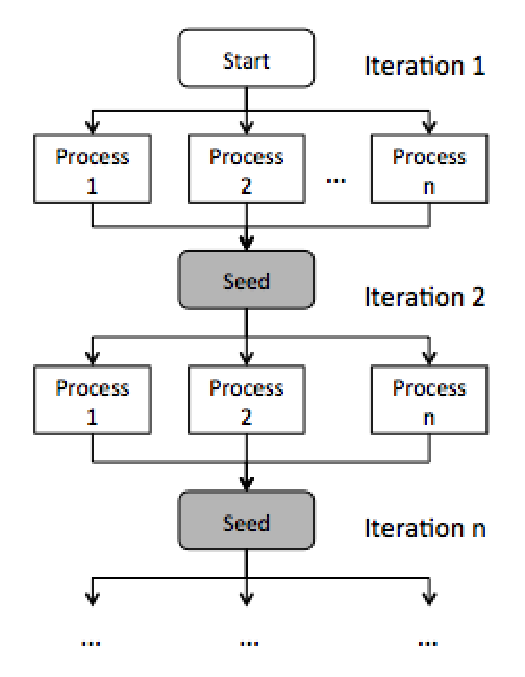
\includegraphics[width=2.9in,height=3.8in]{iterative_sampling}
  \caption{Iterative sampling procedures}
\label{iterative_sampling}
\end{figure}

Motivated by the previous work, we use multiple random restarts and an iterative sampling process to improve decipherment \cite{Dou:2012}, as shown in Figure~\ref{iterative_sampling}. The idea is to start a few sampling processes each with a different random sample. Then we combine the results from different runs and use the combined results to initiate the next sampling iteration. The details of the sampling procedure are listed below:

 \begin{enumerate}
  \item Extract dependency bigrams from parsing outputs and collect their counts.
  \item Keep bigrams whose counts are greater than a threshold $t$. Then start N different randomly seeded and initialized sampling processes. Perform sampling.
  \item At the end of sampling, extract word translation pairs $(f,e)$ from the final sample. Estimate translation probabilities $P(e|f)$  for each pair. Then construct a translation table by keeping translation pairs $(f,e)$ seen in more than one decipherment and use the average $P(e|f)$ as the new translation probability.
  \item Start N different sampling processes again. Initialize the first sample using the translation pairs obtained from the previous step (for each dependency bigram $f_{1},f_{2}$, find an English sequence $e_{1},e_{2}$, whose $P(e_{1}|f_{1})\cdot P(e_{2}|f_{2})\cdot P(e_{1},e_{2})$is the highest). Initialize base distribution with one learned by previous sampling process whose posterior probability is highest. Go to the second step, and repeat until it converges. 
  \item Lower the threshold $t$ to include more bigrams into the sampling process. Go to the second step, and repeat until $t=1$.
 \end{enumerate}

The second step consists of sampling and learning of similarity matrix $M$. The sampling process creates training examples for learning $M$, and the new $M$ is used to update base distribution for future sampling process. In our Spanish-English decipherment experiments, we use 10 different random starts. In experiments, we set $\alpha$ to a small value at the beginning, and gradually increase it  as more ciphtertext becomes available. We set $\alpha$ to 2, 10, and 50 for ciphertexts with 100k, 1 million, and 10 million tokens respectively. 

\section{Deciphering Malagasy}
\label{decipher_malagasy}

%In this section, we first introduce the Malagasy language, and describe the data used in the experiments; then explain what makes deciphering Malagasy more challenging compared with Spanish, and differences in experiment settings for achieving higher decipherment accuracy.
% need to maintain anonymity
%\subsection{The Malagasy Language}

Malagasy belongs to the Malayo-Polynesian branch of the Austronesian language family. Malagasy and English have very different word order, starting with VOS versus SVO. Generally, Malagasy is a typical head-initial language: Determiners precede nouns, while other modifiers and relative clauses follow nouns (e.g. ny ``the'' boky ``book'' mena ``red''). The significant differences in word order pose great challenges for decipherment.


\subsection{Data}

Table~\ref{mlg-en-data} lists the sizes of monolingual and parallel data used in this experiment, released by \newcite{dou-vaswani-knight:2014:EMNLP2014}. The monolingual data in Malagasy contains news text collected from Madagascar websites. The English monolingual data contains Gigaword and additional 300 million tokens of African news. Parallel data (used for evaluation only) is collected from GlobalVoices, a multilingual news website, where volunteers translate news into different languages.

 \begin{table}
 \begin{center}
 \begin{tabular}{ |c|c|c| } \hline
             & Malagasy & English \\ \hline
\multirow{2}{*}{Training} & 16 million & 1.2 billion\\ 
& (Web) & \pbox{2cm}{ (Gigaword \\ and Web)}  \\ \hline
\multirow{2}{*}{Evaluation} & 2.0 million& 1.8 million \\
 & (GlobalVoices) & (GlobalVoices)  \\ \hline
 \end{tabular}
 \caption{Size of data in tokens used in Malagasy-English decipherment experiment. GlobalVoices is parallel data.}
 \label{mlg-en-data}
 \end{center}
 \end{table}
 
\subsection{Systems}
The baseline system is the same as the baseline used in Spanish-English decipherment experiments. We use data provided in previous work \cite{dou-vaswani-knight:2014:EMNLP2014} to build a Malagasy dependency parser. For English, we use the Turbo parser, trained on the Penn Treebank \cite{TurboParser}.  

Because the Malagasy parser does not predict dependency relation types, we use head-child part-of-speech (POS) tag patterns to select a subset of dependency bigrams for decipherment: 
%We list the selected POS tag patterns in Table \ref{mlg-en-dep-type}.

% keep format same as previous section on Spanish.

\begin{itemize}
\item Verb / Noun
\item Verb / Proper Noun
\item Verb / Personal Pronoun
\item Preposition / Noun
\item Preposision / Proper Noun
\item Noun / Adjective
\item Noun / Determiner
\item Noun / Verb Particle
\item Noun / Verb Noun % what is this?
\item Noun / Cardinal
\item Noun / Noun
\end{itemize}

%
% \begin{table}
% \begin{center}
% \begin{tabular}{ |c|c| } \hline
%          Head POS & Child POS \\ \hline
%Verb & Noun \\ \hline
%Verb & Proper Noun \\ \hline
%Verb & Person Pronoun \\ \hline
%Preposition & Noun \\ \hline
%Preposition & Proper Noun \\ \hline
%Noun & Adjective \\ \hline
%Noun & Determiner \\ \hline
%Noun & Verb Particle \\ \hline
%Noun & Verb Noun \\ \hline
%Noun & Cardinal Number \\ \hline
%Noun & Noun \\ \hline
% \end{tabular}
% \caption{Head-Child POS patterns used in decipherment}
% \label{mlg-en-dep-type}
% \end{center}
% \end{table}
%

\subsection{Sampling Procedure}

We use the same sampling protocol designed for Spanish-English decipherment. Compared with Spanish-English decipherment, we find the base distribution plays a more important role in achieving higher decipherment accuracy for Malagasy-English. Therefore, we set weight to 10, 100, and 500 when deciphering 100k, 1 million, and 20 million token ciphtertexts, respectively.


\section{Results}

%
 \begin{table*}[!ht]
 \begin{center}
 \begin{tabular}{ |c|c|c|c|c|c|c|c|c| } \hline
         & \multicolumn{4}{|c|}{Spanish-English} & \multicolumn{4}{|c|}{Malagasy-English} \\ \hline
 Top &  \multicolumn{2}{|c|}{5k} & \multicolumn{2}{|c|}{10k} & \multicolumn{2}{|c|}{5k} & \multicolumn{2}{|c|}{10k} \\ \hline
 System &  Baseline & DMRE & Baseline & DMRE &  Baseline & DMRE & Baseline & DMRE \\ \hline
 100k &  1.9 & 12.4 & 1.1 & 7.1 &  1.2 & 2.7 & 0.6 & 1.4 \\ \hline
 1 million &  7.3 & 37.7& 4.2 & 23.6 &  2.5 & 5.8 & 1.3 & 3.2 \\ \hline
 10 million &  26.0 & 59.0 & 15.9 & 43.7 &  5.4 & 11.2 & 3.0 & 6.9 \\ \hline
 \end{tabular}
 \caption{Spanish-English and Malagasy-English decipherment top-5 accuracy (\%) of 5k and 10k most frequent word types}
 \label{decipher-acc-result}
 \end{center}
 \end{table*}
%

In this section, we first compare decipherment accuracy of the baseline with our new approach, at various ciphertext sizes. Then, we evaluate the quality of the base distribution learned during decipherment.

We use top-5 type accuracy as our evaluation metric.  Given a word type $f$ in Spanish, we find top-5 translation pairs $(f,e)$ ranked by $P(e|f)$ from the learned decipherent translation table. If any pair $(f,e)$ can also be found in a gold translation lexicon $T_{gold}$, we treat the word type $f$ as correctly deciphered. Let $|C|$ be the number of word types correctly deciphered, and $|V|$ be the total number of word types evaluated. We define type accuracy as $\frac{|C|}{|V|}$.

To create $T_{gold}$, we use GIZA to align a small amount of Spanish-English parallel text (1 million tokens for each language), and use the lexicon derived from the alignment as our gold translation lexicon. $T_{gold}$ contains a subset of 4233 word types in the top 5000 frequent word types, and 7479 word types in the top 10k frequent word types. We decipher the 10k most frequent Spanish word types to the 10k most frequent English word types, and evaluate decipherment accuracy on both the 5k most frequent word types as well as the full 10k word types.

 We evaluate accuracy for the 5k and 10k most frequent word types for each language pair, and present them in Table~\ref{decipher-acc-result}.


 \begin{figure}[!ht]
  \centering
  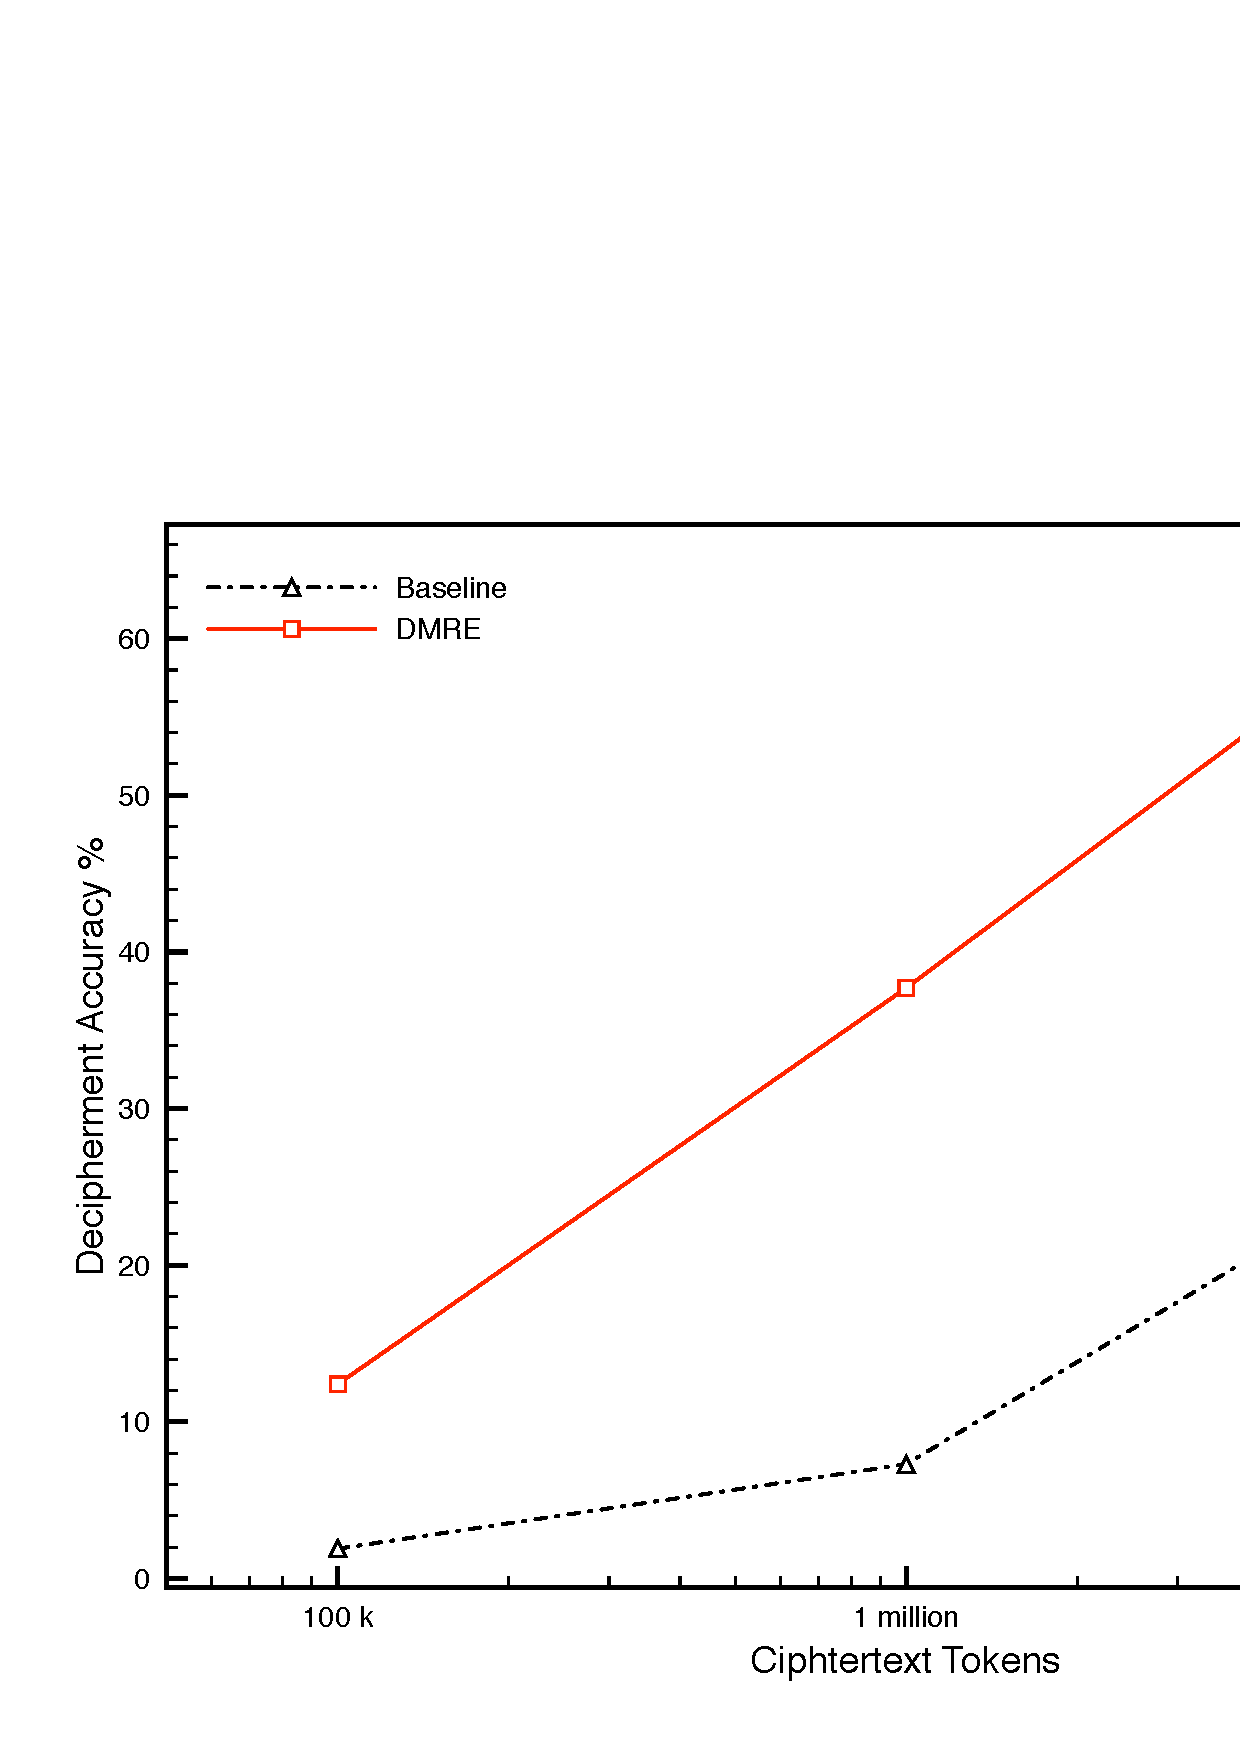
\includegraphics[width=3.1in,height=2.4in]{es_en_curve}
  \caption{Learning curves of top-5 accuracy evaluated on 5k most frequent word types for Spanish-English decipherment.}
\label{es-en-curve}
\end{figure}

We also present the learning curves of decipherment accuracy for 5k most frequent word types. Figure~\ref{es-en-curve} compares the baseline with \textbf{DMRE} in deciphering Spanish into English. Performance of the baseline is in line with previous work \cite{dou-knight:2013:EMNLP}. (The accuracy reported here is higher as we evaluate top 5 accuracy for each word type.) With 100k tokens of Spanish text, the baseline achieves 1.9\% accuracy, while the new system achieves 12.4\% accuracy, which improves the baseline by over 6 times. The improvement holds consistently throughout the experiment. In the end, the baseline achieves 26.0\% accuracy, while the new system achieves 59.0\% accuracy, over 2 times higher. 

 \begin{figure}[!ht]
  \centering
  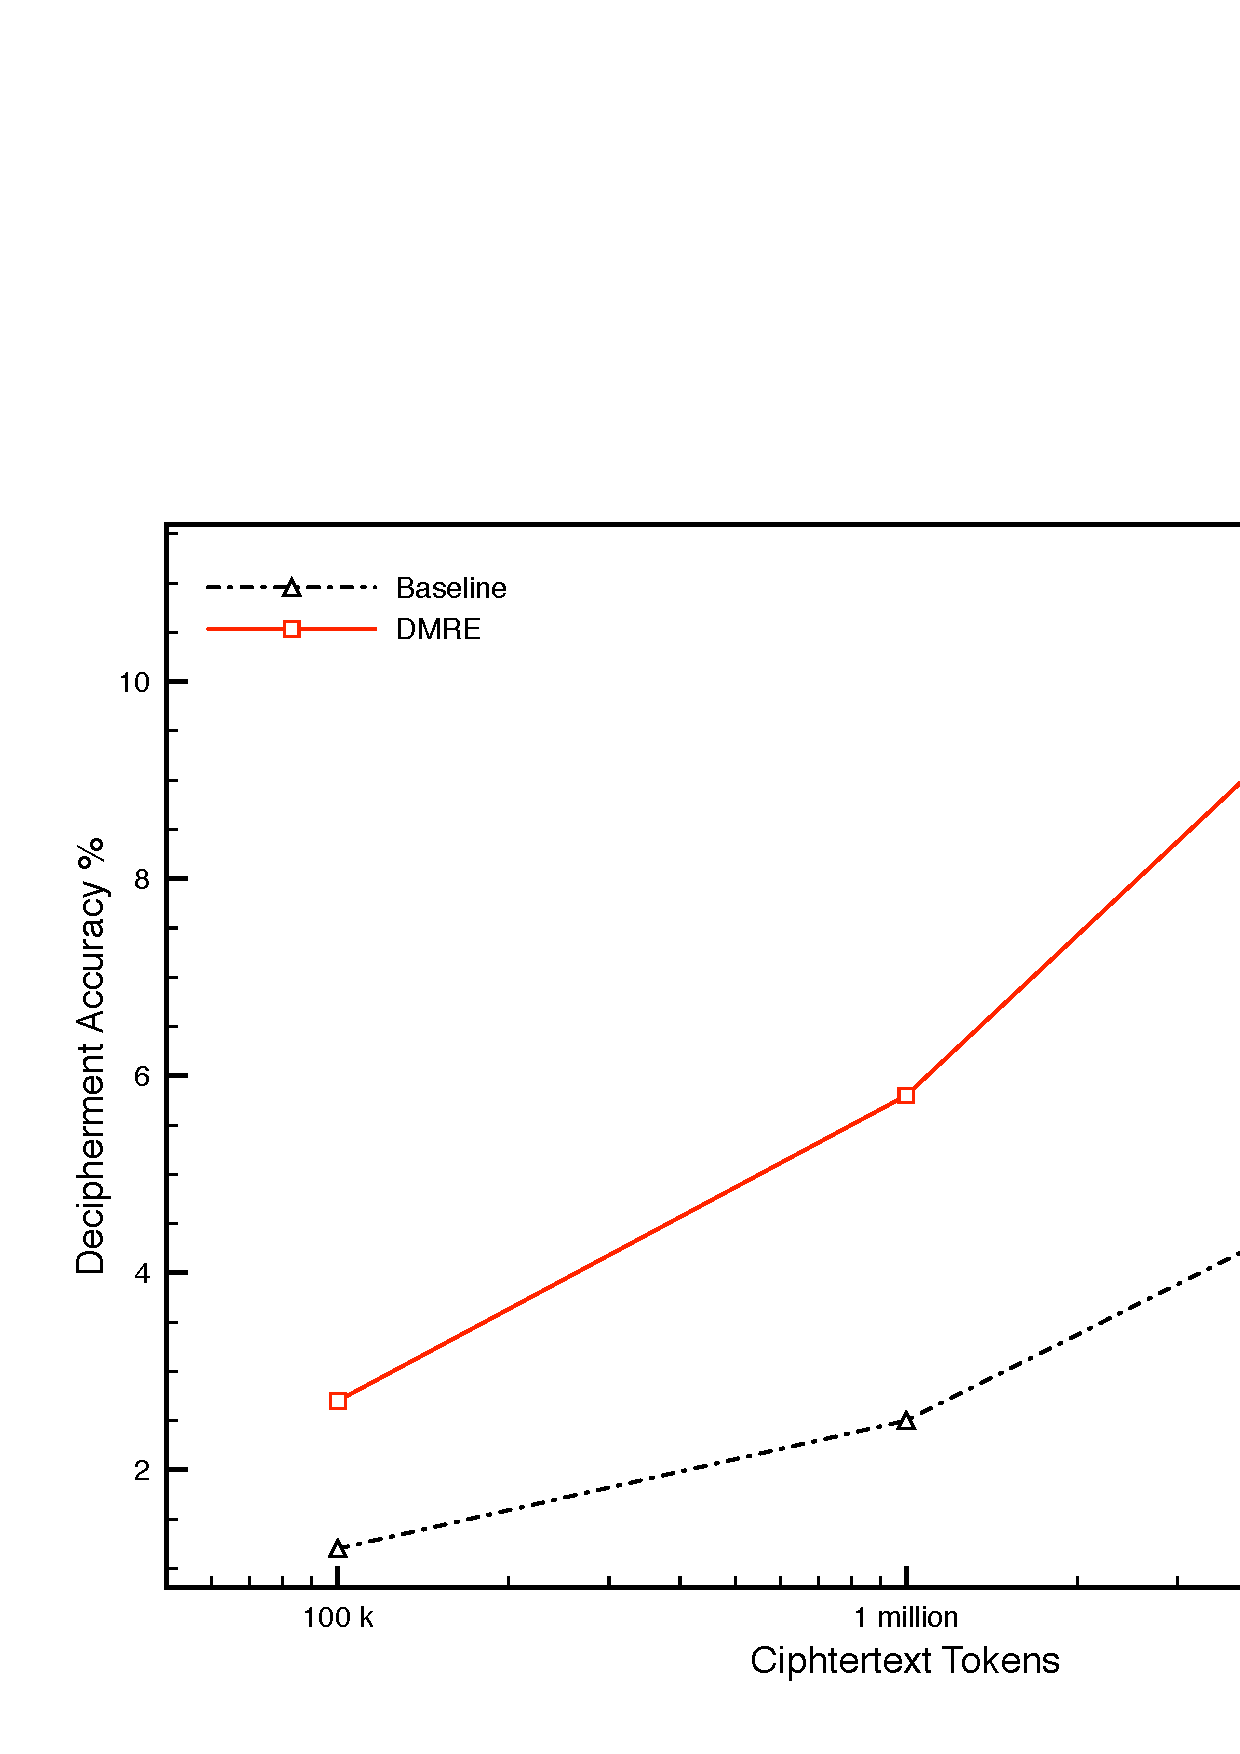
\includegraphics[width=3.1in,height=2.4in]{mlg_en_curve}
  \caption{Learning curves of top-5 accuracy evaluated on 5k most frequent word types for Malagasy-English decipherment.}
\label{mlg-en-curve}
\end{figure}

Figure \ref{mlg-en-curve} compares the baseline with our new approach in deciphering Malagasy into English. With 100k tokens of data, the baseline achieves 1.2\% accuracy, while the new system achieves 2.4\% accuracy.  We observe consistent improvement throughout the experiment. In the end, the baseline accuracy climbs to 5.8\%, while the new system improves it to 11.2\%.

Overall, the improvement we achieved is solid, and is observed across different language pairs. We hypothesize the gain comes from a better base distribution that considers larger context information. This helps prevent the language model driving deicpherment to a wrong direction. 

%We evaluate the base distribution with the same translation table we use for evaluation decipherment accuracy. For each cipher word type $f$, if any of its translation $e$ with score $P(e|f) \geq 0.1$ appears in the top 500 candidates proposed by the base distribution, we view that the base distribution proposes a correct translation for $f$. We evaluate base distribution learned during Spanish-English decipherment. The total number of evaluable word types is 7469. With 100k cipher tokens, 5416 are correct, with 10m cipher tokens, 6123 are correct.
To show that the base distribution we learned is sensible , we visualize it in Figure \ref{viz_countries} and Figure \ref{viz_close}. To generate the visualizations, we first project English embeddings vectors into Spanish embeddings space using the similarity matrix $M$. Then, we put the word vectors together and project all of them from 50 dimension down to 2 dimension. Two words are close if their embeddings vectors are similar. Ideally, we hope words that are translations are also close to each other.

 \begin{figure}[!ht]
  \centering
  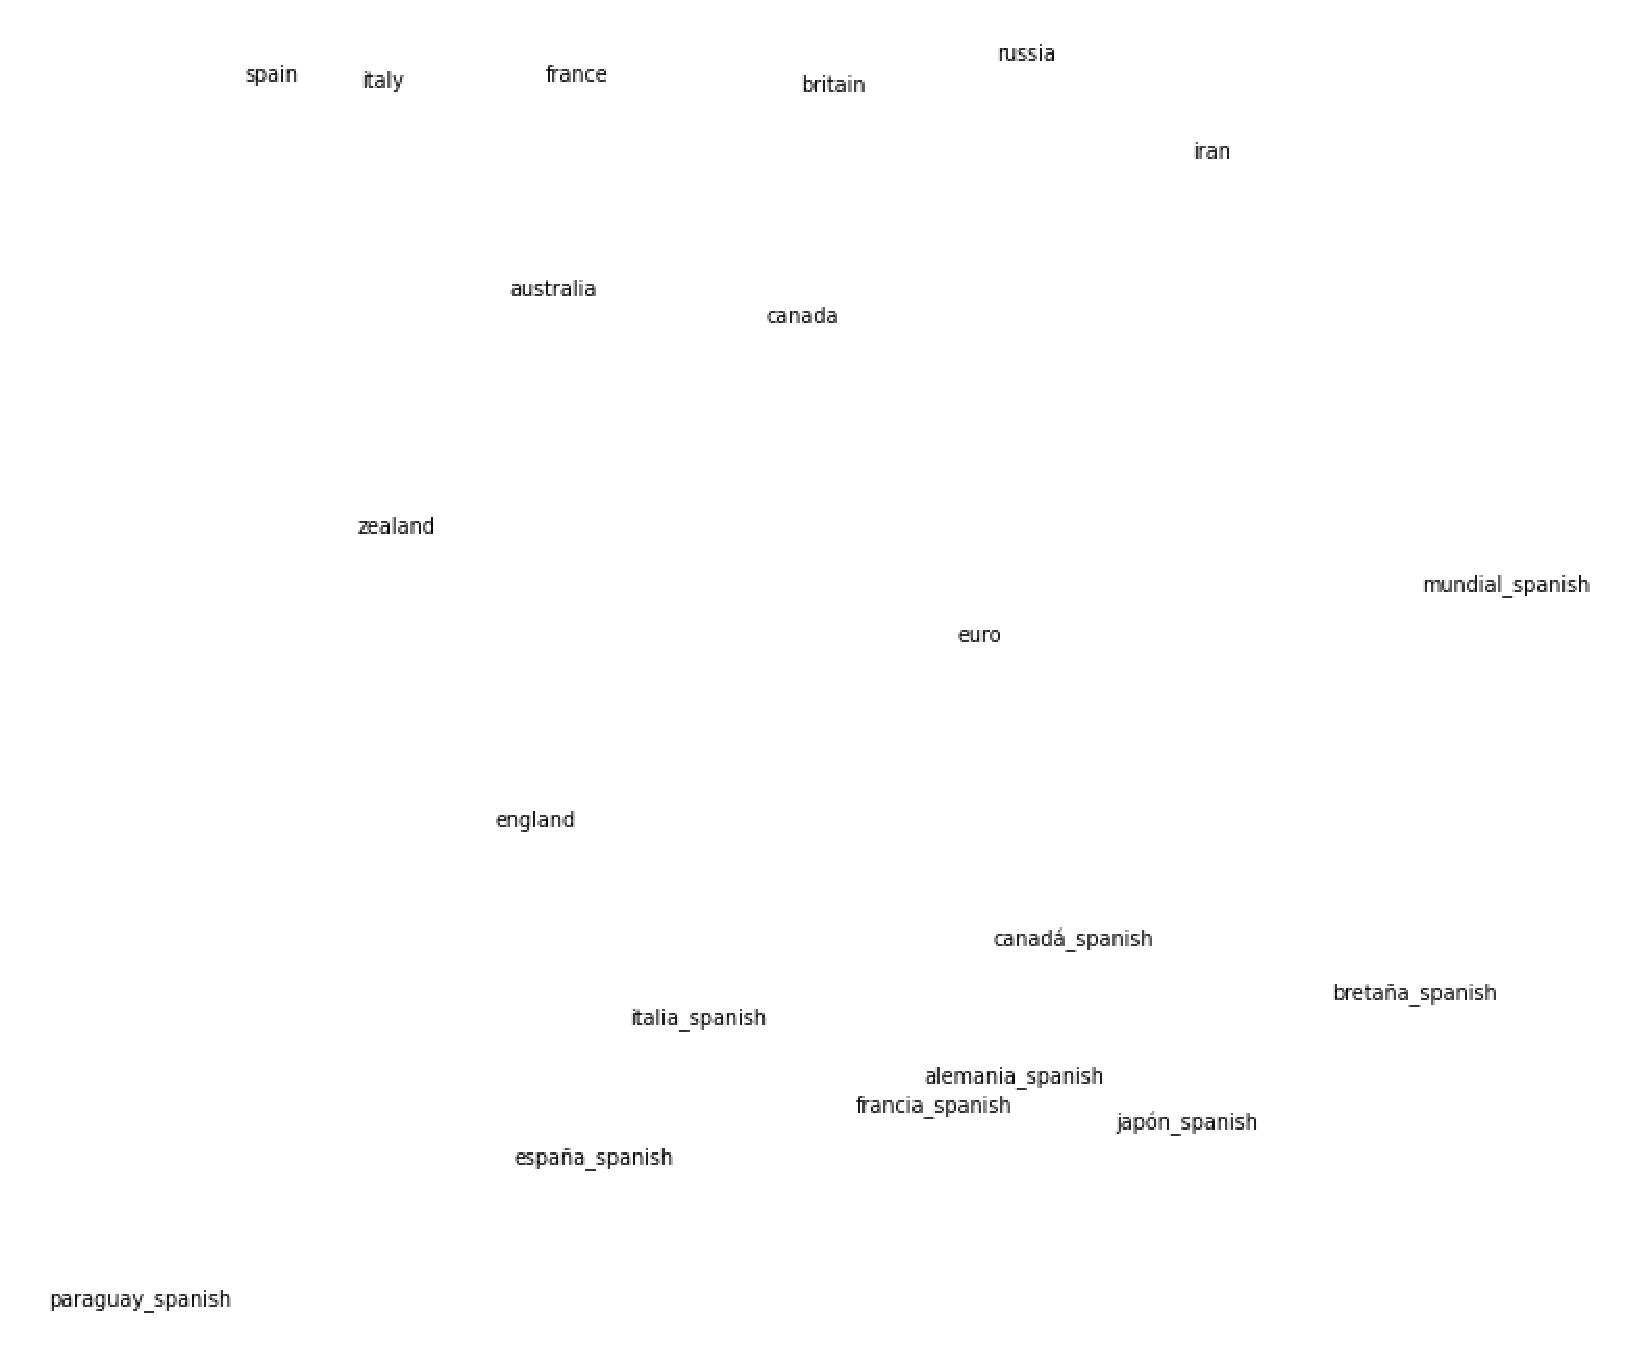
\includegraphics[width=2.5in,height=2.5in]{viz_countries}
  \caption{A snapshot of visualization from mapping of 1k most frequent English words to Spanish words. Groups of country names in Spanish and English are close.}
\label{viz_countries}
\end{figure}

The first thing we observe is that translations appear close as groups. As shown in 
Fiture \ref{viz_countries}, the group of country names in Spanish and their English translations are near to each other.


 \begin{figure}[!ht]
  \centering
  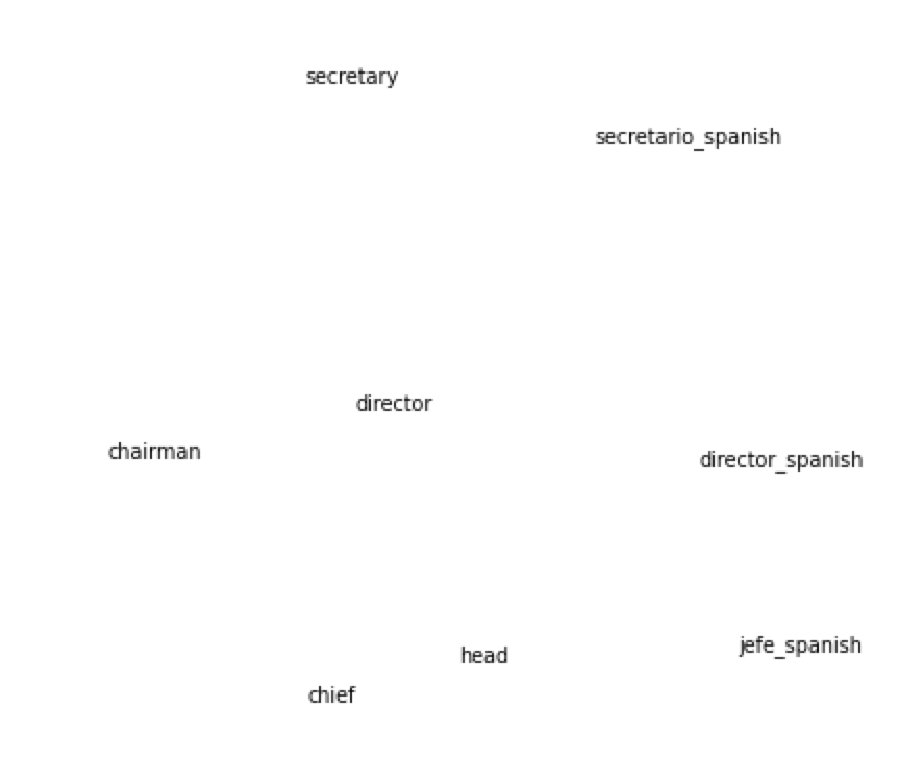
\includegraphics[width=2.5in,height=2.5in]{viz_top1000}
  \caption{A snapshot of visualization from mapping of 1k most frequent English words to Spanish words. Pairs of translations that are right next to each other.}
\label{viz_close}
\end{figure}

As shown in Figure \ref{viz_close} When we look deeper, we also find many pairs of translations that are right next to each other. Previous work has also produced similar visualization with help of parallel data. However, we learn the mapping using only monolingual data.

\section{Conclusion and Future Work}

We propose a new framework that simultaneously performs decipherment and learns a cross-lingual mapping of word embeddings. Our method is both theoretically sound and practically powerful. The mapping is used to give decipherment a better base distribution. 

Experimental results show that our new algorithm improves state-of-the-art decipherment accuracy significantly: from 29\% to 64.7\% for Spanish/English, and 5.1\% to 11.2\% for Malagasy/English. This improvement could lead to further advances in using monolingual data for to improve end-to-end MT.
In the future, we will work on making the new method scale to much larger vocabulary sizes, and apply it to improve MT systems.
\section*{Acknowledgments}
This work was supported by ARL/ARO (W911NF-10-1-0533) and DARPA (HR0011-12-C-0014).



\bibliography{ref}
\bibliographystyle{acl}

\end{document}